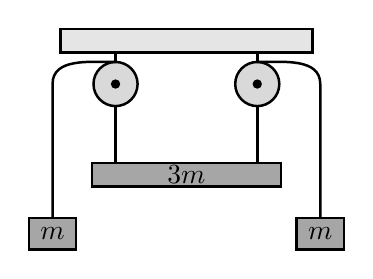
\begin{tikzpicture}[line width=0.9pt]
  % ceiling
  \draw[fill=black!10] (-1.6,3.0) rectangle (1.6,3.3);
  % two pulleys
  \draw[fill=black!15] (-0.9,2.6) circle (0.28);
  \filldraw (-0.9,2.6) circle (1.2pt);
  \draw[fill=black!15] (0.9,2.6) circle (0.28);
  \filldraw (0.9,2.6) circle (1.2pt);
  % strings from ceiling to pulleys
  \draw (-0.9,3.0) -- (-0.9,2.88);
  \draw (0.9,3.0) -- (0.9,2.88);
  % strings from pulleys down to central bar
  \draw (-0.9,2.32) -- (-0.9,1.6);
  \draw (0.9,2.32) -- (0.9,1.6);
  % central bar of mass 3m
  \draw[fill=black!35] (-1.2,1.3) rectangle (1.2,1.6);
  \node at (0,1.45) {$3m$};
  % strings over pulleys down to side masses
  \draw (-0.9,2.88) to[out=180,in=90] (-1.7,2.6) -- (-1.7,0.9);
  \draw (0.9,2.88) to[out=0,in=90] (1.7,2.6) -- (1.7,0.9);
  % side masses
  \draw[fill=black!35] (-2.0,0.5) rectangle (-1.4,0.9);
  \node at (-1.7,0.7) {$m$};
  \draw[fill=black!35] (1.4,0.5) rectangle (2.0,0.9);
  \node at (1.7,0.7) {$m$};
\end{tikzpicture}
